
\FloatBarrier
\newpage
\section{Application Android SmartCanton Manager}
\label{sec-soft_android}


L'application Android, nommée SmartCanton Manager, a pour but de créer un pont entre deux technologies, comme illustré en \cref{fig-diagram_android_architecture} mais également de créer un canal d'échange sécurité pour le transfert de l'AppKey LoRaWAN. 

L'application offre également la possibilité de tester les différents capteurs présents sur une DevBox en se connectant aux différents services Bluetooth présentés en \cref{sec-software_ble_services}. La récupération des données s'effectue à l'aide de lectures BLE ou via des flux de notifications BLE.

\begin{figure}[ht!]
    \centering
    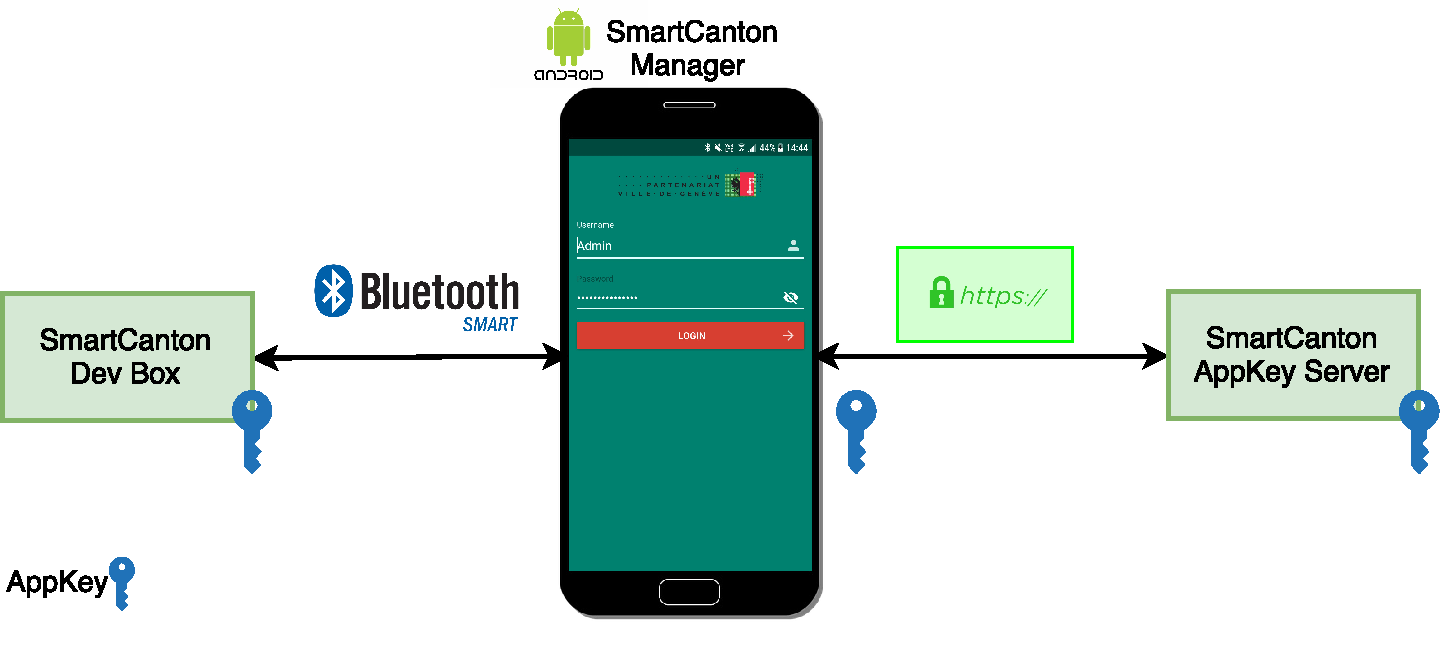
\includegraphics[width=1.0\textwidth]{Figures/Software/diagram_android_architecture.pdf}
    \caption{Rôle de l'application mobile}
    \label{fig-diagram_android_architecture}
\end{figure}


\subsection{Frameworks utilisés}

Afin d'accélérer la programmation sur Android, deux frameworks majeurs ont été utilisés. Ceux-ci sont listés dans les sous-sections qui suivent.

\subsubsection{SweetBlue}

Android est censé s'abstraire du matériel afin d'offrir une interface générique pour chaque plateforme utilisée, surtout sur les smartphones. Néanmoins, le comportement du Bluetooth diffère encore entre les différents périphériques Android utilisés. Par exemple, Samsung bride la fréquence des scans Bluetooth possible sur ses smartphones lorsque ceux-ci sont verrouillés. Cette décision a été prise pour réduire la consommation énergétique des applications qui s'exécutent en arrière-plan sur un smartphone. Ceci n'est pas le cas sur la plupart des autres constructeurs. La \textit{stack} Bluetooth sur Android est également très \textit{bas niveau}. Par exemple, si on souhaite lire plusieurs caractéristiques BLE à la suite, l'utilisateur doit lui-même créer une file de lecture avec la gestion de toutes les erreurs, car deux lectures ne peuvent pas être effectuées en parallèle. Voici une liste complète des divers problèmes qui sont aujourd'hui encore non résolus sur les diverses versions d'Android :
\begin{center}
    \url{https://github.com/iDevicesInc/SweetBlue/wiki/Android-BLE-Issues}
\end{center}

Pour pallier à cela, une bibliothèque nommée SweetBlue a été développée par l'entreprise iDevicesInc\footnote{\url{https://idevicesinc.com/sweetblue/}}. Celle-ci a pour but de simplifier l'intégration du Bluetooth dans une application et d'essayer de corriger certaines instabilités. La bibliothèque est gratuite dans son intégralité pour un usage privé même si l'application finale n'est pas vendue à des utilisateurs.


\subsubsection{Retrofit}

Sur Android, la gestion des appels asynchrones peut vite devenir compliquée et répétitive. Retrofit est un client \textit{type-safe} pour les API REST sur Java, avec un accent prononcé pour Android. Cette bibliothèque est développée par l'entreprise Square\footnote{\url{http://square.github.io/retrofit/}}, spécialisée dans les logiciels \textit{open sources}. Cette bibliothèque fournit un framework complet et simple à utiliser pour interagir avec les APIs et recevoir des requêtes avec le client OkHttp\footnote{\url{http://square.github.io/okhttp/}}.

La gestion des erreurs HTTP sont directement traitées par le framework à l'aide de \textit{callbacks} avec les méthodes \texttt{success} et \texttt{failure}.


\subsection{Manuel d'utilisation de l'application}

L'\cref{AppendixAndroidAppUserGuide} contient un manuel d'utilisation de l'application Android. Avec toutes les étapes qui sont nécessaires pour se connecter au serveur, lister les périphériques Bluetooth à proximité, ainsi que la connexion avec ces derniers.


\subsection{Activités}

 Pour ne pas surcharger la présentation de cette section, toutes les captures d'écran de l'application sont présentées dans le manuel d'utilisateur situé à l'\cref{AppendixAndroidAppUserGuide}.
 
 
\begin{figure}[ht!]
    \centering
    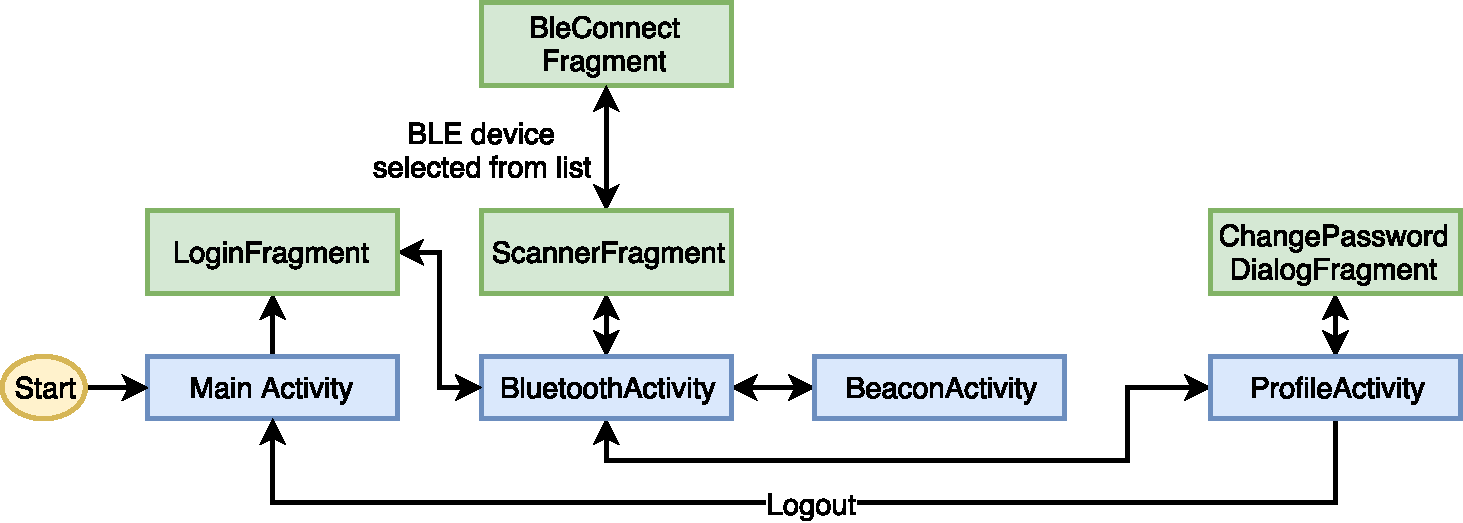
\includegraphics[width=1.0\textwidth]{Figures/Software/diagram_android_activites.pdf}
    \caption{Diagramme d'interconnexions entre les différentes activités Android}
    \label{fig-diagram_android_activites}
\end{figure}


L'architecture générale de l'application avec la présentation des diverses activités et fragments est visible sur la \cref{fig-diagram_android_activites}. On constate que l'application n'est composée que de quatre activités. Voici leurs différents rôles :
\begin{itemize}
    \item \texttt{MainActivity} : affiche le fragment \texttt{LoginFragment} qui offre la possibilité à l'utilisateur de s'authentifier auprès du serveur, afin de recevoir un \textit{token} JWT (cf. \cref{fig_apdx-login_activity}). Une fois le login accepté, l'activité \texttt{BluetoothActivity} est appelée.
    \item \texttt{BluetoothActivity} : gère les diverses communications Bluetooth entre les différents périphériques. Cette activité peut afficher deux fragments :
        \begin{enumerate}
            \item \texttt{ScannerFragment} : fragment instancié par défaut au démarrage de l'activité et a pour but de lister tous les périphériques Bluetooth Low Enerny à proximité (cf. \cref{fig_apdx-bluetooth_scanner_frag}). Les dispositifs sont affichés dans une liste et peuvent être sélectionnés par l'utilisateur.
            \item \texttt{BleConnectFragment} : fragment affiché lorsque l'utilisateur sélectionne un périphérique. Lors du chargement du fragment, une requête vers le serveur est automatiquement envoyée afin de savoir si le dispositif est connu en fonction de l'adresse MAC de ce dernier. Si le périphérique est connu, l'utilisateur peut se connecter au périphérique via Bluetooth et ainsi accéder aux divers périphériques (cf. \cref{fig_apdx-ble_dev_connection_process}). Il peut également mettre à jour le périphérique avec les dernières configurations LoRaWAN contenues sur le serveur.
        \end{enumerate}
    \item \texttt{BeaconActivity} : ne contient pas de fragment, car elle n'a qu'un seul et unique rôle, qui est de générer un certain nombre de \textit{beacons} afin de simuler des périphériques Bluetooth Low Energy à proximité comme vu en \cref{sec-software_scanner_ble}.
    \item \texttt{ProfileActivity} : Cette activité permet d'afficher les informations sur l'utilisateur connecté, ainsi que sur le \textit{token} JWT récupéré lors de la connexion. Ici l'utilisateur peut également se déconnecter de sa session (cf. \cref{fig_apdx-profile_activity}).
\end{itemize}



\subsection{Sécurité}


Pour ce qu'il s'agit de la sécurité, tout est directement géré par Android même. Dans le cas des requêtes HTTPS, il suffit de spécifier que l'URL du serveur est en HTTPS pour que toute la communication soit automatiquement chiffrée à l'aide du certificat fournit par le serveur. \\

Dans le cas du Bluetooth, c'est le périphérique qui décide du mode de sécurité qu'il accepte (cf. \cref{sec-security_ble}). Android s'occupe donc d'effectuer la connexion avec requêtes de celui-ci. La demande de \textit{passkey} est demandée directement par l'OS et ne peut pas être directement validée par l'application. Pour informer l'utilisateur sur la présence du \textit{passkey}, une popup est affichée lors de la connexion dévoilant ainsi le PIN que l'utilisateur doit rentrer sur le périphérique (cf. \cref{fig_apdx-ble_dev_connected_startup}).

